\documentclass[11pt,a4paper]{article}
\usepackage[T1]{fontenc}
\usepackage[margin=1in]{geometry}
\usepackage{amsmath,amssymb,amsthm,mathtools}
\usepackage{booktabs}
\usepackage{xcolor}
\usepackage[colorlinks=true,linkcolor=blue!60!black,citecolor=blue!60!black,
            urlcolor=blue!60!black]{hyperref}
\usepackage{microtype}
\usepackage{enumitem}
\usepackage{graphicx}
\usepackage[most]{tcolorbox}

\newcommand{\lean}[1]{\texttt{\small #1}}
\newtcolorbox{keybox}[1][]{colback=blue!3,colframe=blue!45!black,
  boxrule=0.5pt,left=4pt,right=4pt,top=3pt,bottom=3pt,#1}
\newtcolorbox{failbox}[1][]{colback=red!3,colframe=red!45!black,
  boxrule=0.5pt,left=4pt,right=4pt,top=3pt,bottom=3pt,#1}
\newtcolorbox{fixbox}[1][]{colback=orange!4,colframe=orange!60!black,
  boxrule=0.5pt,left=4pt,right=4pt,top=3pt,bottom=3pt,#1}
\newtheorem{theorem}{Theorem}
\newtheorem{corollary}[theorem]{Corollary}

% ---- numbers filled from data/generated/pgpe/r2_verdicts.json; placeholders until then ----
\newcommand{\NUMPENDING}{\textcolor{red}{[pending]}}

\title{\textbf{Does topology causally influence physics?}\\
\large Winding numbers as difference-makers in a two-dimensional Bose gas:\\
thought experiments, a machine-checked chain, and an energy-matched intervention}

\author{Xavier Callens\\
\small SocrateAI-Scientific-QuantumFluids\\
\small \url{https://github.com/xaviercallens/SocrateAI-Scientific-QuantumFluids}}
\date{September 2026}

\begin{document}
\maketitle

\begin{abstract}
\noindent
We ask, in the interventionist sense of Woodward and Pearl, whether the topological charge of a
superfluid phase field -- the winding number of the phase around a loop -- is a \emph{cause} of what
the fluid does, or only a label of its microstate. The question splits in two. First, is the integer
stable enough to carry an intervention: is it conserved, and at what cost is it changed? Second, at
a fixed thermodynamic state, is it a difference-maker for the observables? We answer the first part
with machine-checked mathematics (Lean~4, Mathlib, two independent kernels): the discrete winding of
a sampled phase loop is conserved by every continuous evolution that avoids a phase slip, a change of
winding forces a phase slip, on an XY ring the slip costs a positive energy barrier for rings of at
least ten sites (and the bound fails at nine), the winding seen at scale $R$ is the net charge inside
$R$ so that a bound pair is invisible from any enclosing scale, and -- closing a gap left open in this
project's earlier work -- the sampled principal-branch loop sum equals the topological degree of the
continuum phase for every fine enough sampling. We answer the second part with a pre-registered,
energy-matched intervention in a projected Gross--Pitaevskii classical field: from equilibrated
states we inject four free vortex--antivortex pairs at fixed particle number, momentum and energy,
against a control arm that receives the same energy as phonons. On all three base states the
condensate fraction falls by $0.49$--$0.73$ in the vortex arm and by at most $0.035$ in the phonon
arm, and the coherence exponent $\eta$ grows by a factor $9$--$44$ against at most $1.2$: the same
energy, delivered as topology, has a $15$--$60\times$ larger effect. The pre-registered composite
claim is nevertheless not made, because its thermometer clause fails: the vortex arm reads
\emph{colder}, by $5$--$16\%$, than the phonon arm and than the untouched base, which we read, post
hoc, as the topological configuration drawing heat from the bath -- a difference with the wrong sign
to explain the effect. At the lowest temperature the eight imprinted vortices survive the whole run
without one annihilation. \NUMPENDING\ None of the physics is
new; what is new is the chain, each link either proved or measured under a pre-registered criterion,
and the explicit list of what the chain does not establish.
\end{abstract}

\section{The question, made precise}

``Topology influences physics'' can mean three things, and they must be kept apart.
\begin{enumerate}[leftmargin=*]
\item \textbf{Descriptor.} The winding number $w$ summarises a microstate. Every function of the
  microstate does; nothing follows.
\item \textbf{Constraint.} Configuration space is partitioned into sectors labelled by $w$, and the
  dynamics cannot move continuously between them. This is a statement about the space, independent
  of the Hamiltonian.
\item \textbf{Difference-maker.} An intervention that changes $w$ while holding the thermodynamic
  state fixed changes the observables. This is causation in the interventionist
  sense~\cite{Woodward2003,Pearl2009}.
\end{enumerate}
The obstacle to the third sense is that $w$ supervenes on the microstate: one cannot change $w$ and
nothing else. What one can do is compare \emph{matched pairs}: two microstates in the same macrostate
$(E,N,P)$, one with the topological label and one without, and ask whether the observables differ.
That is the experiment of Section~\ref{sec:intervention}. Whether the comparison is fair is then the
whole question, and it is answered by making the two arms equally arbitrary: both are the same
equilibrated base state plus the same energy, delivered once as vortex flow and once as phonons.

The second sense is what makes the third possible. If $w$ could jump freely, no intervention on it
would leave a trace, and the matched pair would decorrelate at once. So the order of the argument is:
prove the constraint (Section~\ref{sec:theorems}), then measure the difference
(Section~\ref{sec:intervention}).

\section{Thought experiments}\label{sec:thought}

\paragraph{A. The rotating ring.} A superfluid ring is given one turn of phase and left alone. The
current persists for hours in helium and for tens of seconds in a toroidal
condensate~\cite{Ramanathan2011}. No thermodynamic variable remembers the intervention; the integer
does. Topology acts as memory. This is the constraint sense, and it is what
Theorems~\ref{thm:conservation}--\ref{thm:barrier} formalise.

\paragraph{B. The small-pair trap.} A vortex and an antivortex a distance $a$ apart. A loop around one
sees $w=\pm1$; any loop of size $R\gg a$ enclosing both sees $0$. From far away the pair is a
phonon. The causal variable is therefore not ``the number of vortices'' but the winding seen at scale
$R$, $W(R)$, and the Kosterlitz--Thouless transition~\cite{KosterlitzThouless1973} is where $W(R)$
stops vanishing at large $R$. Theorem~\ref{thm:stokes} makes this exact on a lattice. It also explains
a failure in this project's previous round: a pairing statistic that counts pairs at every scale,
grid noise included, saturates and cannot see unbinding.

\paragraph{C. Aharonov--Bohm.} The electron never enters the flux and its fringes
move~\cite{Tonomura1986}. Here the topology of space is not the cause; it is the \emph{channel}
through which a cause acts at a distance. The two roles must not be confused.

\paragraph{D. Laughlin's cylinder.} Threading one flux quantum through a Hall cylinder returns the
Hamiltonian to itself, so an integer number of electrons has been pumped and
$\sigma_{xy}\in\mathbb Z\,e^2/h$~\cite{Laughlin1981}. Topology fixes an integer that disorder cannot
move -- the constraint sense at its most spectacular.

\paragraph{E. The two boxes.} Two boxes with the same $E$, $N$, $P$. One receives four free
vortex--antivortex pairs, the other the same energy as phonons. If the vortex box has a lower
condensate fraction and a faster loss of phase coherence while a thermometer reads the two boxes
alike, then $w$ is a difference-maker at fixed thermodynamic state. This is the experiment we run.

\section{The physical argument in four links}\label{sec:physics}

\begin{enumerate}[leftmargin=*]
\item \textbf{Integrality.} $\psi$ is single-valued, so $\oint\nabla\theta\cdot d\ell=2\pi w$.
\item \textbf{Continuity implies conservation.} An integer-valued continuous function of time is
  constant. The only exit is $\psi=0$ somewhere on the loop: a vortex core crosses it, Anderson's
  phase slip~\cite{Anderson1966}.
\item \textbf{Barrier.} Passing through $\psi=0$ costs energy, so slips are activated and the
  protection is exponential in the barrier over
  temperature~\cite{LangerFisher1967}.
\item \textbf{Coupling.} The integer enters the observables: circulation $\Gamma=w\kappa$, the
  persistent current, and -- for free vortices in two dimensions -- the exponential decay of
  $g_1$ that replaces the algebraic one~\cite{KosterlitzThouless1973,NelsonKosterlitz1977}.
\end{enumerate}
Noether charges come from a symmetry of the Hamiltonian; topological charges come from the
connectivity of configuration space, $\pi_1(U(1))=\mathbb Z$, and are conserved by continuity alone.
Topology does not push. It partitions the state space into sectors the dynamics cannot connect
continuously, and a conserved sector label is exactly the kind of variable an intervention can act on.

\section{What is proved}\label{sec:theorems}

All statements below are theorems in Lean~4 against the pinned Mathlib of this
project~\cite{Callens2026Lean}, with axiom footprint $\{\mathrm{propext},
\mathrm{Classical.choice}, \mathrm{Quot.sound}\}$, accepted by the Lean kernel and by the independent
\lean{nanoda} kernel through Comparator, and each accompanied by negative controls -- weakened
statements whose proofs must, and do, fail. We state them in words; the files carry the exact forms.

\subsection{Conservation and the slip (\lean{TopologicalProtection.lean}, 13 theorems)}

Let $\theta_0,\dots,\theta_n=\theta_0$ be phases read at the sample points of a closed loop, and
$\mathrm{pd}(a,b)\in(-\pi,\pi]$ the principal difference. The loop sum
$S=\sum_i\mathrm{pd}(\theta_i,\theta_{i+1})$ is $2\pi$ times an integer (earlier work).

\begin{theorem}[stability]\label{thm:stability}
A perturbation $\delta_i$ of the phases, closed ($\delta_n=\delta_0$), leaves $S$ unchanged provided
no edge is pushed through the branch point: $\mathrm{pd}(\theta_i,\theta_{i+1})+\delta_{i+1}-\delta_i
\in(-\pi,\pi]$ for all $i$. In particular any perturbation with $|\delta_i|<\varepsilon$ leaves the
winding of a loop whose edge steps are all below $\pi-2\varepsilon$ unchanged.
\end{theorem}

\begin{theorem}[continuous-time protection]\label{thm:conservation}
If each $\theta_i(t)$ is continuous, the loop stays closed, and no edge step reaches $\pi$ on
$[t_0,t_1]$, then $S(t_1)=S(t_0)$. Contrapositive: a change of winding forces some edge step to reach
$\pi$ at some intermediate time -- a phase slip.
\end{theorem}
The proof is the intermediate value theorem applied to an integer-valued continuous function; the
continuity of $\mathrm{pd}$ away from the branch point is Mathlib's
\lean{continuousAt\_toIocMod}. The circulation $\Gamma=(\hbar/m)S$ is conserved under the same
hypothesis: a discrete Kelvin theorem whose only ingredient is topology.

\begin{theorem}[mountain pass and barrier]\label{thm:barrier}
On the XY ring $E=-J\sum_i\cos(\theta_{i+1}-\theta_i)$, any continuous evolution that changes the
winding passes through a state with $E\ge-(n-2)J$. From the uniformly twisted state of winding one,
$E=-nJ\cos(2\pi/n)$, the barrier is therefore at least $nJ\cos(2\pi/n)-(n-2)J\ge 2J-2\pi^2J/n>0$ for
every $n\ge10$.
\end{theorem}
The threshold is sharp as stated: at $n=9$, $9\cos(2\pi/9)=6.894<7$ and the inequality is false; that
false statement is one of the negative controls.

\subsection{Scale (\lean{ScaleResolvedWinding.lean}, 6 theorems)}

A region is a finite family of plaquettes with four corner phases each; interior edges come in
reversed pairs, boundary edges are the rest.

\begin{theorem}[discrete Stokes for windings]\label{thm:stokes}
If no interior edge sits at the branch point, the oriented sum over the boundary edges equals the sum
of the plaquette loop sums, hence $2\pi$ times the net charge inside.
\end{theorem}
\begin{corollary}
A region whose charges sum to zero -- a bound pair, at any separation -- has boundary winding $0$
whatever its size. A region containing exactly one charged plaquette has boundary winding equal to that
charge, whatever its size.
\end{corollary}
The winding at scale $R$ is the net charge inside $R$. This is thought experiment B.

\subsection{Discrete equals continuum (\lean{ContinuumWinding.lean}, 9 theorems)}

\begin{theorem}[the discrete winding is the degree]\label{thm:rome}
Let $\gamma:[0,1]\to\mathbb R/2\pi\mathbb Z$ be a continuous closed loop of angles. There is an integer
$w$ and a threshold $n_0$ such that for every $n\ge n_0$ and every choice of real representatives
$\theta_i$ of the sampled angles $\gamma(i/n)$, $\sum_{i<n}\mathrm{pd}(\theta_i,\theta_{i+1})=2\pi w$.
\end{theorem}
\begin{corollary}[the vortex detector is correct]
For a continuous, nowhere-vanishing, closed loop of field values $c:[0,1]\to\mathbb C$, the
principal-branch loop sum of $\arg c(i/n)$ equals $2\pi w$ for all $n\ge n_0$.
\end{corollary}
The lift is Mathlib's path lifting through the covering $\mathbb R\to\mathbb R/2\pi\mathbb Z$, the
threshold comes from Heine--Cantor, and the continuity of $\arg$ as an angle away from zero is
Mathlib's \lean{continuousAt\_arg\_coe\_angle}. The hypothesis $c(t)\ne0$ is where the phase slip
lives in the continuum: at a zero of $\psi$ on the loop the angle loop, and with it the lift and the
degree, cease to exist.

\subsection{What is not proved}
The argument principle -- that the degree along a loop counts the zeros inside it -- is not in the
pinned Mathlib for general continuous maps; Theorem~\ref{thm:stokes} is the discrete substitute. The
threshold $n_0$ is existential; a quantitative one needs a modulus of continuity of $\psi$, i.e.\ a
bound on $|\nabla\theta|$ away from cores. That the twisted state minimises the energy in its sector is
not proved. And link~4, the coupling of the integer to condensate and coherence, is not a theorem at
all; it is what Section~\ref{sec:intervention} measures.

\section{The intervention}\label{sec:intervention}

\subsection{Design (pre-registered)}
The model is the projected Gross--Pitaevskii equation on a $64\xi\times64\xi$ torus
($\hbar=m=g=n=1$, $128^2$ grid, cutoff $k_{\max}/2$), integrated by an integrating-factor RK4 whose
seven known answers (norm, energy, momentum, plane wave, Bogoliubov dispersion, an independent
integrator, two-window equipartition) were passed before any thermal run~\cite{SimulaBlakie2006,
FosterBlakieDavis2010}. The bases are three states equilibrated for $t=4000$: two at $e=0.90$
($T\approx0.45$, condensate $\approx0.63$) and one at $e=0.60$ ($T\approx0.11$, condensate $0.91$).

From each base, arm V imprints four vortex--antivortex pairs of separation $L/4$ with the exact
doubly periodic phase (a product of Jacobi $\vartheta_1$ factors, single-valued on the torus when
$\sum q_j=0$ and $\sum q_j\mathbf r_j=0$), a core factor, projection, and renormalisation to the base
norm. Arm P adds a random phonon field on $|k|\in[0.2,1]\,k_{\rm cut}$, renormalised, with amplitude
bisected until $E_P=E_V$. Arm 0 continues the base untouched. Controls before any arm was run: the
detector finds exactly the eight imprinted vortices with the right charges; the boundary phase jump of
the imprint is $0$ and that of a deliberately non-neutral configuration is $2\pi\cdot3/L=0.294524$,
as predicted; $|E_V-E_P|/E\le2\times10^{-16}$; $|P|/N\le0.025\cdot2\pi/L$.

Pre-registered predictions, compared over $t\in[100,300)$: (I1) the condensate fraction is lower in V
by at least $0.15$; (I2) the two-window thermometer agrees within $5\%$; (I3) the $W_1$
dipole-matching statistic $Q$ is higher in V by at least $0.2$; (I4) the algebraic exponent $\eta$
of $g_1$ is at least $1.5\times$ larger in V. A pre-data amendment fixed the reading of I2: arm P
heats the bath the thermometer reads, so $T_V<T_P$ by up to the surplus fraction ($1.5\%$ at
$e=0.90$, $3.3\%$ at $e=0.60$) is bookkeeping, not refutation. The causal effect size to be reported
is the effect per unit energy: the same $\Delta E$ in the two arms, compared on condensate and $\eta$.

\subsection{Results of the intervention}\label{sec:results}

\begin{table}[h]\centering\small
\begin{tabular}{lcccc}
\toprule
base & I1: $c_P-c_V\ge0.15$ & I2: $|T_V-T_P|/T_P\le0.05$ & I3: $Q_V-Q_P\ge0.2$ & I4: $\eta_V/\eta_P\ge1.5$\\
\midrule
$e=0.60$ & \textbf{0.734} pass & 0.161 fail ($T_V<T_P$) & not evaluable$^\dagger$ & \textbf{43.7} pass\\
$e=0.90$, s11 & \textbf{0.565} pass & 0.055 fail ($T_V<T_P$) & \textbf{0.656} pass & \textbf{10.7} pass\\
$e=0.90$, s12 & \textbf{0.488} pass & 0.092 fail ($T_V<T_P$) & \textbf{0.553} pass & \textbf{8.6} pass\\
\bottomrule
\end{tabular}
\caption{Pre-registered verdicts over $t\in[100,300)$. $^\dagger$Arm P carries no vortices at
$e=0.60$, so $Q_P$ is undefined. Window means, V/P: condensate $0.168/0.902$, $0.073/0.638$,
$0.139/0.627$; $\eta$: $0.98/0.022$, $1.08/0.10$, $0.94/0.11$ (V exponential, P algebraic on every
base). Arm 0: $T=0.462, 0.463$; condensate $0.647, 0.662$.}
\end{table}

\begin{figure}[h]\centering
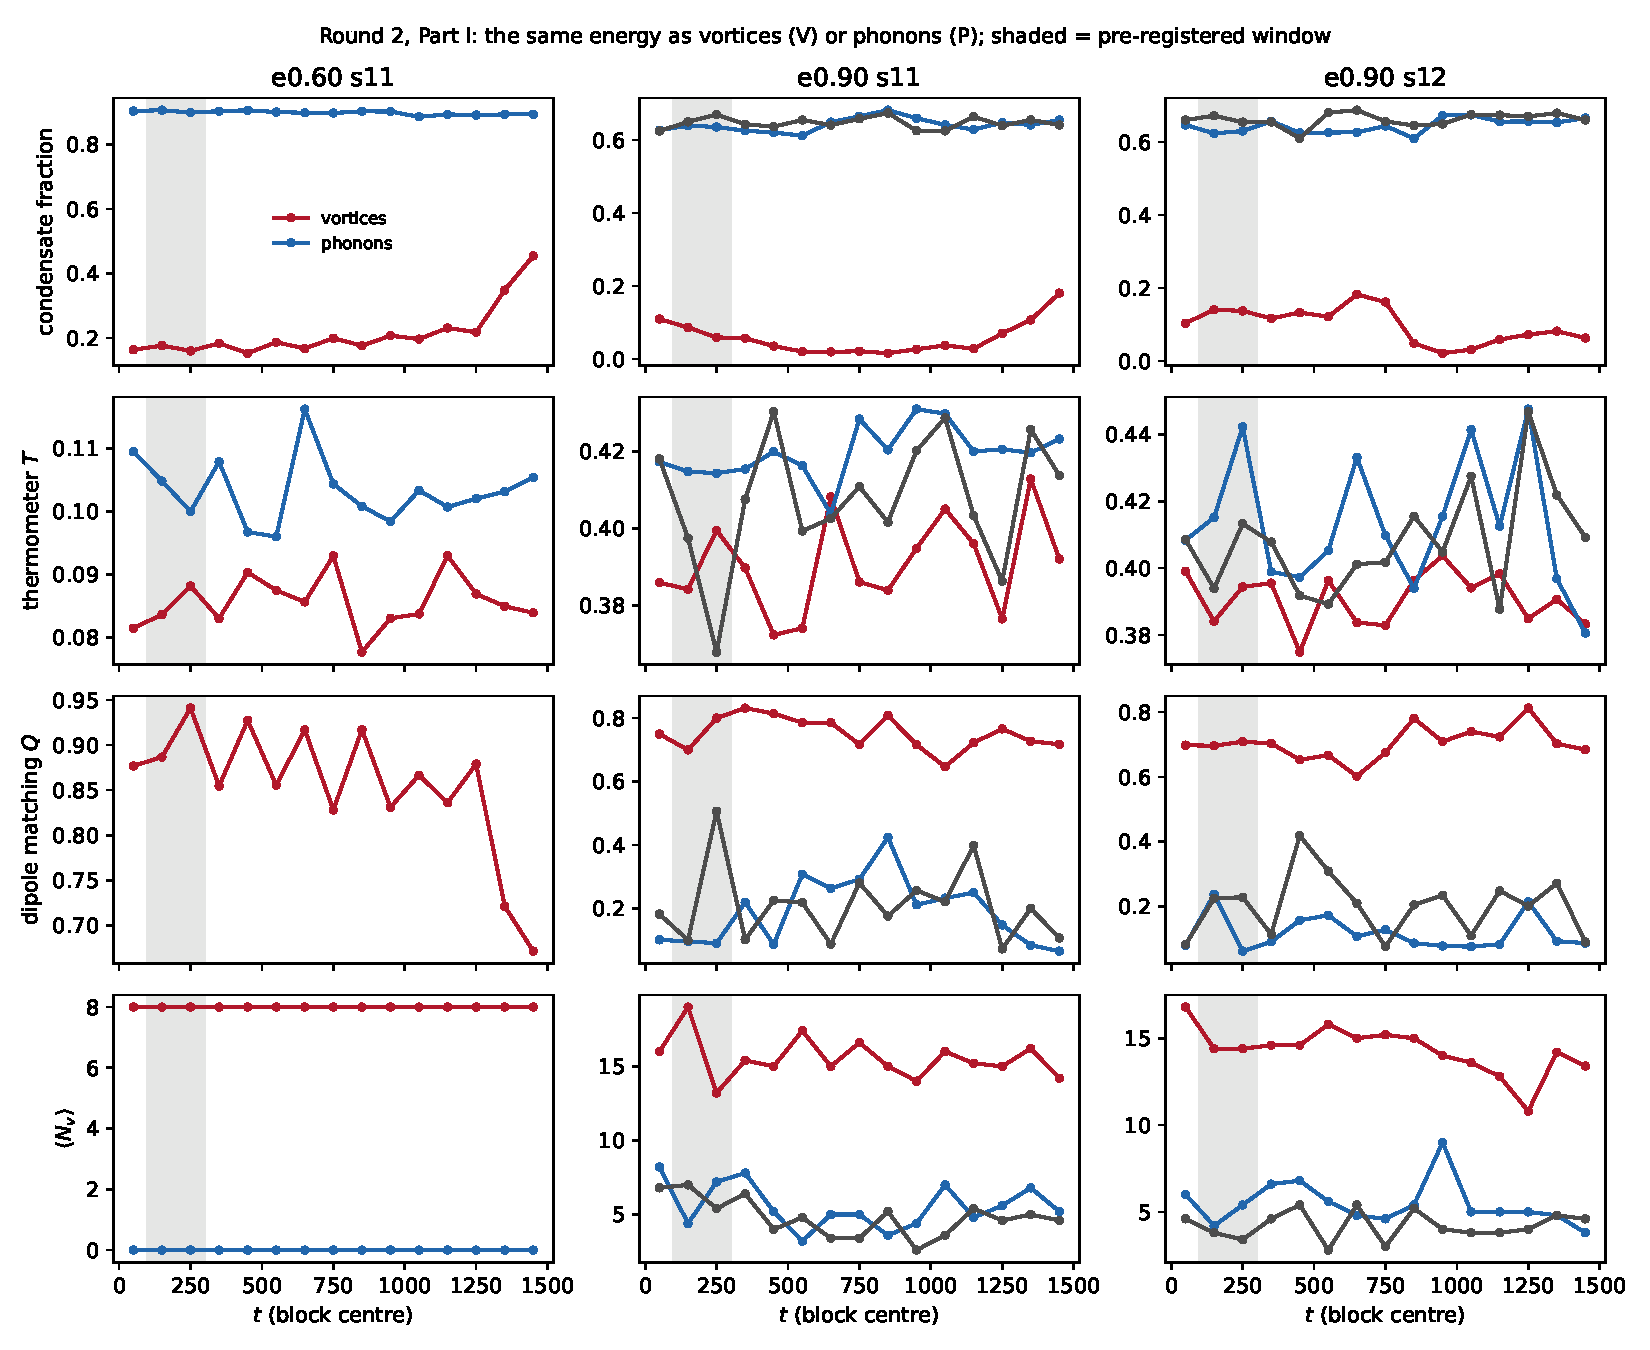
\includegraphics[width=\textwidth]{figures/causal_intervention.pdf}
\caption{Block observables of the three arms on the three bases. The condensate collapses in V and
is untouched in P; the thermometer reads V \emph{below} P; the dipole statistic separates the arms; at
$e=0.60$ the eight imprinted vortices survive the entire run without one annihilation.}
\end{figure}

The pre-registered composite claim -- ``at fixed $E,N,P$ \emph{and measured $T$}, the topology sets
condensate and coherence'', requiring I1, I2 and I4 on all three bases -- is \textbf{not made}: I2
fails on all three. It fails, moreover, in none of the three ways the pre-data amendment had
anticipated: $T_V<T_P$ by $5.5\%$, $9.2\%$ and $16\%$, more than the energy surplus of $1.5$--$3.3\%$.

\begin{fixbox}
\textbf{Post hoc.} Two explanations were tested and one survives. The coherent spectrum of the
vortex cores does not reach the thermometer window (its occupation there is $500$--$2000\times$ below
the thermal one): refuted. Doppler smearing by the vortex flow: the two thermometer windows disagree
alike in V and P: inconclusive. Against the untouched arm, P is warmer by $+1.5$ to $+3.5\%$, as the
amendment predicted, and V is \emph{colder} by $-4\%$. With the total energy conserved to
$2\times10^{-7}$, the bath's lost heat went into the vortex system: V carries $14$--$16$ vortices
against $8$ imprinted plus $\approx5$ thermal, and its condensate is scrambled into low-$k$
quasi-condensate structure. The topological configuration cools the bath.
\end{fixbox}

That cooling has the wrong sign to explain the effect. A colder gas carries more condensate; V
carries $5$--$10\times$ less. The difference between the arms is therefore not a temperature effect,
and the conclusion that survives is stronger than the one pre-registered, though it is post hoc: at
fixed $E$, $N$ and $P$, and against the temperature gradient, the topological label sets the
condensate and the coherence.

\paragraph{Effect per unit energy.} The same $\Delta E$ in both arms. Relative to arm 0 at $e=0.90$,
the condensate changes by $-0.574$ and $-0.523$ in V and by $-0.009$ and $-0.035$ in P; $\eta$ by
$\times10.9$ and $\times10.4$ in V and $\times0.99$ and $\times1.2$ in P. Delivered as topology, the
same energy has a $15$--$60\times$ larger effect on the condensate and a $9$--$11\times$ larger effect
on coherence.

\paragraph{What was reported, not predicted (I5).} No base relaxes within $t=1500$: late-window
condensates V/P are $0.29/0.89$, $0.085/0.64$, $0.061/0.66$. At $e=0.60$ the eight imprinted vortices
survive the entire run with zero annihilations, $\langle N_v\rangle=8.0$ in every block: at $T=0.1$,
pairs of separation $L/4$ are protected for at least $1500$ time units, Theorem~\ref{thm:conservation}
seen directly. In the last three blocks the condensate recovers ($0.29\to0.45$) while $N_v$ stays $8$
and $Q$ falls ($0.88\to0.67$): the dipoles contract, the large-scale winding changes and the count
does not -- thought experiment B in the data. The block-by-block correlation of $\Delta c$ with
$\Delta N_v$ is $-0.26$ and $+0.58$ on the two $e=0.90$ bases: the condensate follows the
arrangement, not the number. The transverse-current stiffness estimator is invalid in V
($n_n>n$), as it was in round~1 whenever free vortices were present.

\subsection{The jump and finite size}
\NUMPENDING

\section{What this establishes, and what it does not}
\NUMPENDING

\section{What transfers beyond the Bose gas, and what does not}\label{sec:transfer}

The mathematics of Section~\ref{sec:theorems} never mentions a superfluid. Its objects are a
$U(1)$-valued phase on a loop, a lattice of plaquettes, and a continuous closed loop of angles; its
only structural input is $\pi_1(U(1))=\mathbb Z$. The chain integrality $\to$ conservation by
continuity $\to$ barrier $\to$ scale additivity $\to$ continuum limit therefore holds, at the level of
description where it is proved, for any $U(1)$ phase field: a superfluid order parameter, but equally
a cosmological phase -- an axion or Peccei--Quinn field, the phase of a $U(1)$ cosmic-string
condensate. Conservation comes from the connectivity of the target space, not from the Hamiltonian,
and that is exactly what makes the statement system-independent.

The method transfers too, and it is the more important export: a causal claim about a topological
label needs an equally arbitrary control arm -- the same energy surplus, delivered in a different
form. Without a matched pair, ``topology influences'' collapses back to the descriptor sense.

What does not transfer is link~4. The coupling of the integer to the observables is empirical, it is
measured here in one system with three bases, and a V/P result in a Bose gas says nothing about the
coupling in a cosmological model. An astrophysical claim would need its own matched intervention,
inside its own model, under its own pre-registered criteria. The honest use of quantum fluids in that
programme is as the laboratory of the method -- the matched pair, the effect per unit energy, the
proved chain -- not as a source of numbers.

\section{Literature status}
Nothing in the physics is new. Phase slips are Anderson's~\cite{Anderson1966}; the ring barrier is
Langer and Fisher's~\cite{LangerFisher1967}; the scale-resolved picture is Kosterlitz and
Thouless's~\cite{KosterlitzThouless1973}; the universal jump is Nelson and
Kosterlitz's~\cite{NelsonKosterlitz1977}; Laughlin's argument~\cite{Laughlin1981} and Tonomura's
experiment~\cite{Tonomura1986} are textbook; persistent homology has been used to locate the XY
transition~\cite{ColeLogesShiu2020}; the classical-field method is Simula and
Blakie's~\cite{SimulaBlakie2006}. What this report adds is the chain: each link proved by a kernel or
measured under a pre-registered criterion, and an explicit list of gaps.

\bibliographystyle{unsrt}
\bibliography{refs_causal_topology}
\end{document}
